\begin{frame}{$d(K^-, n)$ reaction and J-PARC E31}
  \begin{tabular}{cc}
    \begin{minipage}{0.65\hsize}
      Using bubble chamber at the CERN by Braun \cite{Braun}. \\
      $\blacktriangleright$ 686-848 $MeV/$c $K^-$ beam. \\
      $\blacktriangleright$ Wide angle of $n$ was measured. \\
      $\Rightarrow$ Diag.(a) is considered to be dominant. \\
      
      J-PARC E31 experiment\\
      $\blacktriangleright$ 1.0 $GeV/$c $K^-$ beam. \\
      $\blacktriangleright$ Super-forward neutron was measured. \\
      $\Rightarrow$ Diag.(b) is considered to be dominant.
      
      \begin{thebibliography}{99}
        \scriptsize
      \bibitem{Braun} \href{https://www.sciencedirect.com/science/article/pii/0550321377900153}
        {O. Braun et el., Nucl. Phys. B {\bf 129}, 1 (1977).}
      \end{thebibliography}
    \end{minipage}
 
    \begin{minipage}{0.35\hsize}
      \begin{figure}[htbp]
        \centering
        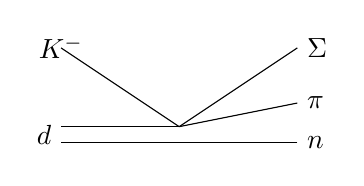
\begin{tikzpicture}
          \draw (-1.5,    1) node {$K^-$}--(0,    0);
          \draw (-1.5,    0)--(0,    0);
          \draw (-1.5, -0.2)--(0, -0.2);
          
          \node (d) at (-1.5, -0.1) [left] {$d$};
          
          \draw ( 1.5,  1.0) node [right] {$\Sigma$} -- (0,    0);
          \draw ( 1.5,  0.3) node [right] {$\pi$}    -- (0,    0);
          \draw ( 1.5, -0.2) node [right] {$n$}      -- (0, -0.2);
        \end{tikzpicture}
        \\
        (a) 1-step reaction
          
        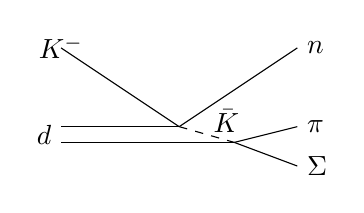
\begin{tikzpicture}
          \draw (-1.5,    1) node {$K^-$}--(0,    0);
          \draw (-1.5,    0)--(0,    0);
          \draw (-1.5, -0.2)--(0.7, -0.2);
          \node (d) at (-1.5, -0.1) [left] {$d$};
          
          \draw (0, 0) -- (0.7, -0.2) [dashed];
          \node (barK) at (0.6, -0.2) [above] {$\bar{K}$};
          
          \draw ( 1.5,  -0.5) node [right] {$\Sigma$} -- (0.7, -0.2);
          \draw ( 1.5,  -0.0) node [right] {$\pi$}    -- (0.7, -0.2);
          \draw ( 1.5,  1.0) node [right] {$n$}      -- (0,    0);
        \end{tikzpicture}
        \\
        (b) 2-step reaction
      \end{figure}
    \end{minipage}
  \end{tabular}
\end{frame}
